\chapter{Soporte del Simulado Robot LEGO Ev3}
\chaptermark{Soporte simulado}
\label{chap:simulado}
Ahora que tenemos definidos cuáles van a ser nuestros objetivos y la infraestructura que vamos a utilizar para llevarlos acabo, en este capítulo se va a hablar del proceso de integración en la plataforma del robot simulado. Primero se describe cómo se ha materializado el \textit{LEGO EV3} en el simulador \textit{WebSim} de la plataforma \textit{Kibotics}. Después se describe la implementación realizada de la interfaz de programación a través de la cual el estudiante recoge las lecturas de los sensores simulados u ordena movimiento a los motores simulados. Finalmente , a modo de validación experimental, se presentan los tres ejercicios desarrollados que utilizan esa interfaz de programación del robot simulado.. Pero antes de eso se darán unas nociones básicas de las características de este robot, para poder entender, el proceso de desarrollo. 
\section{Modelo 3D}
\label{sec:Modelo}
Para simular el robot, el primer paso es crear un modelo tridimensional que puedas incluir en el entrono de \textit{A-Frame}. Para ello se ha utilizado la aplicación de \textit{Blender}, primero, busqué en el almacén Web (propio de la plataforma) un modelo del \textit{Bloque Ev3} al que le pudiera insertar, los modelos de los brazos delanteros, sensores y piezas sueltas necesarias para completar el modelo de \textit{Robot Lego Base}.

 \begin{figure}[H]
    \centering
    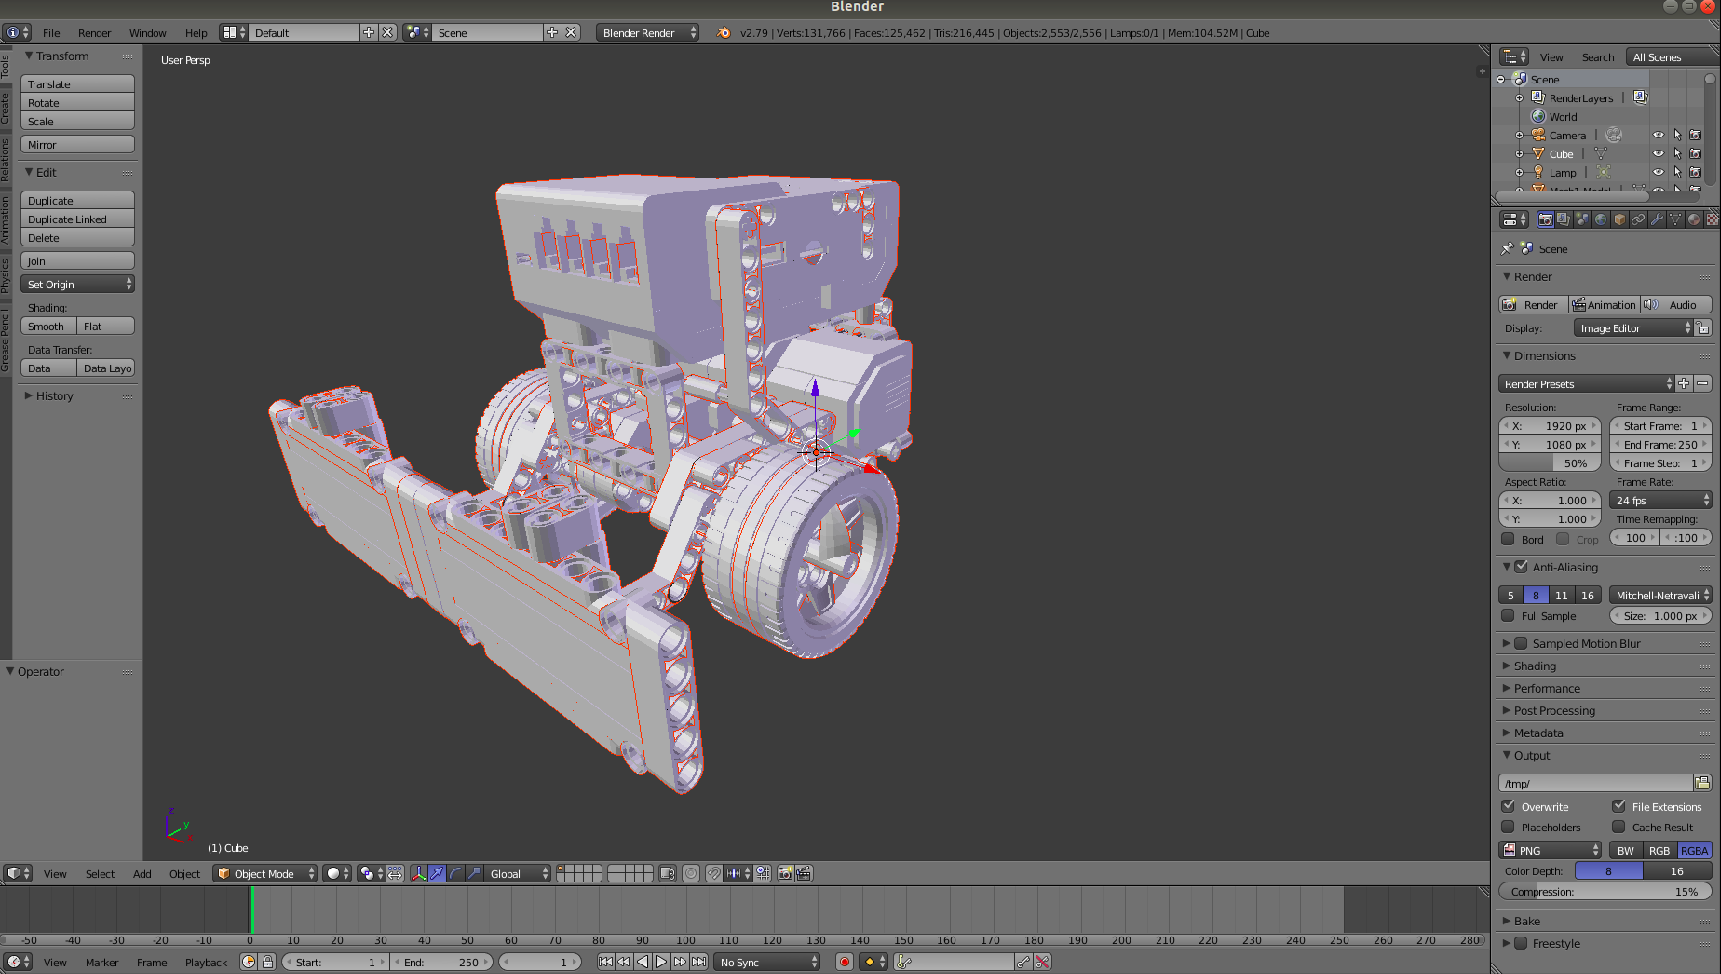
\includegraphics[width=0.7\textwidth]{img/primermodelo.png}
    \caption{Robot base} \label{fig:primer}
\end{figure}

Una vez creado este modelo, el número de aristas era demasiado alto al estar formado por muchos pequeños modelos de piezas, y hace que el modelo completo, pese demasiado, y los tiempos de carga sean demasiado largos. Además de que en \textit{Blender} existen focos de luz, que crean reflejos en el modelo, que no son necesarios para la implementación en \textit{A-Frame}. \newline

Para solucionar esto y mejorar el modelo se realizan las siguiente modificaciones:


\begin{itemize}
\item Reducción del número de polinomios para reducir el número de aristas.
\item Cambiar las texturas reflectantes por texturas mates.
\item Dar color al robot imitando los colores del \textit{LEGO EV3} real. 
\end{itemize}


Una vez realizados estos cambios se procede a insertar en el modelo tridimensional simulado los tres tipos de sensores que incluye el robot \textit{LEGO EV3} y los cambios en el modelo que sean necesarios para que tenga sentido la instalación del sensor.
\\

  \begin{figure}[H]
    \centering
    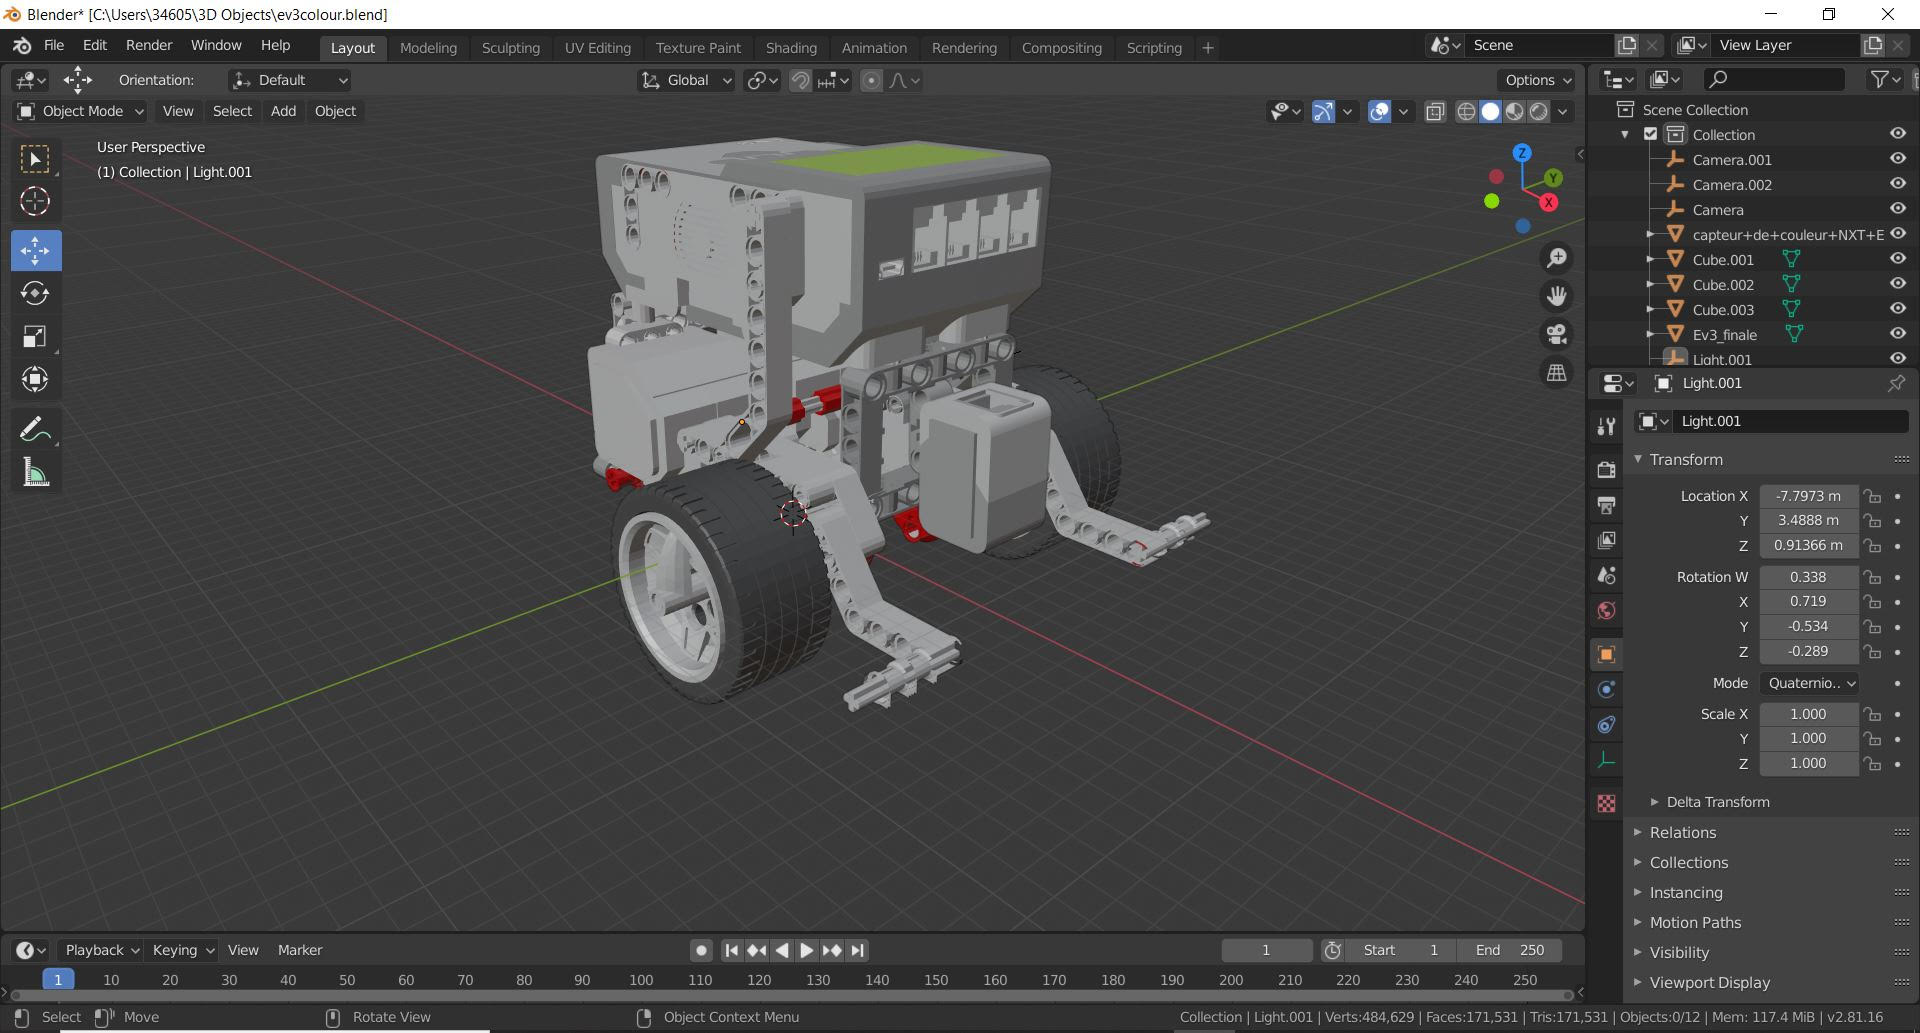
\includegraphics[width=0.7\textwidth]{img/blendercolor.jpg}
    \caption{Robot con sensor de color} \label{fig:color}
\end{figure}
 \begin{figure}[H]
    \centering
    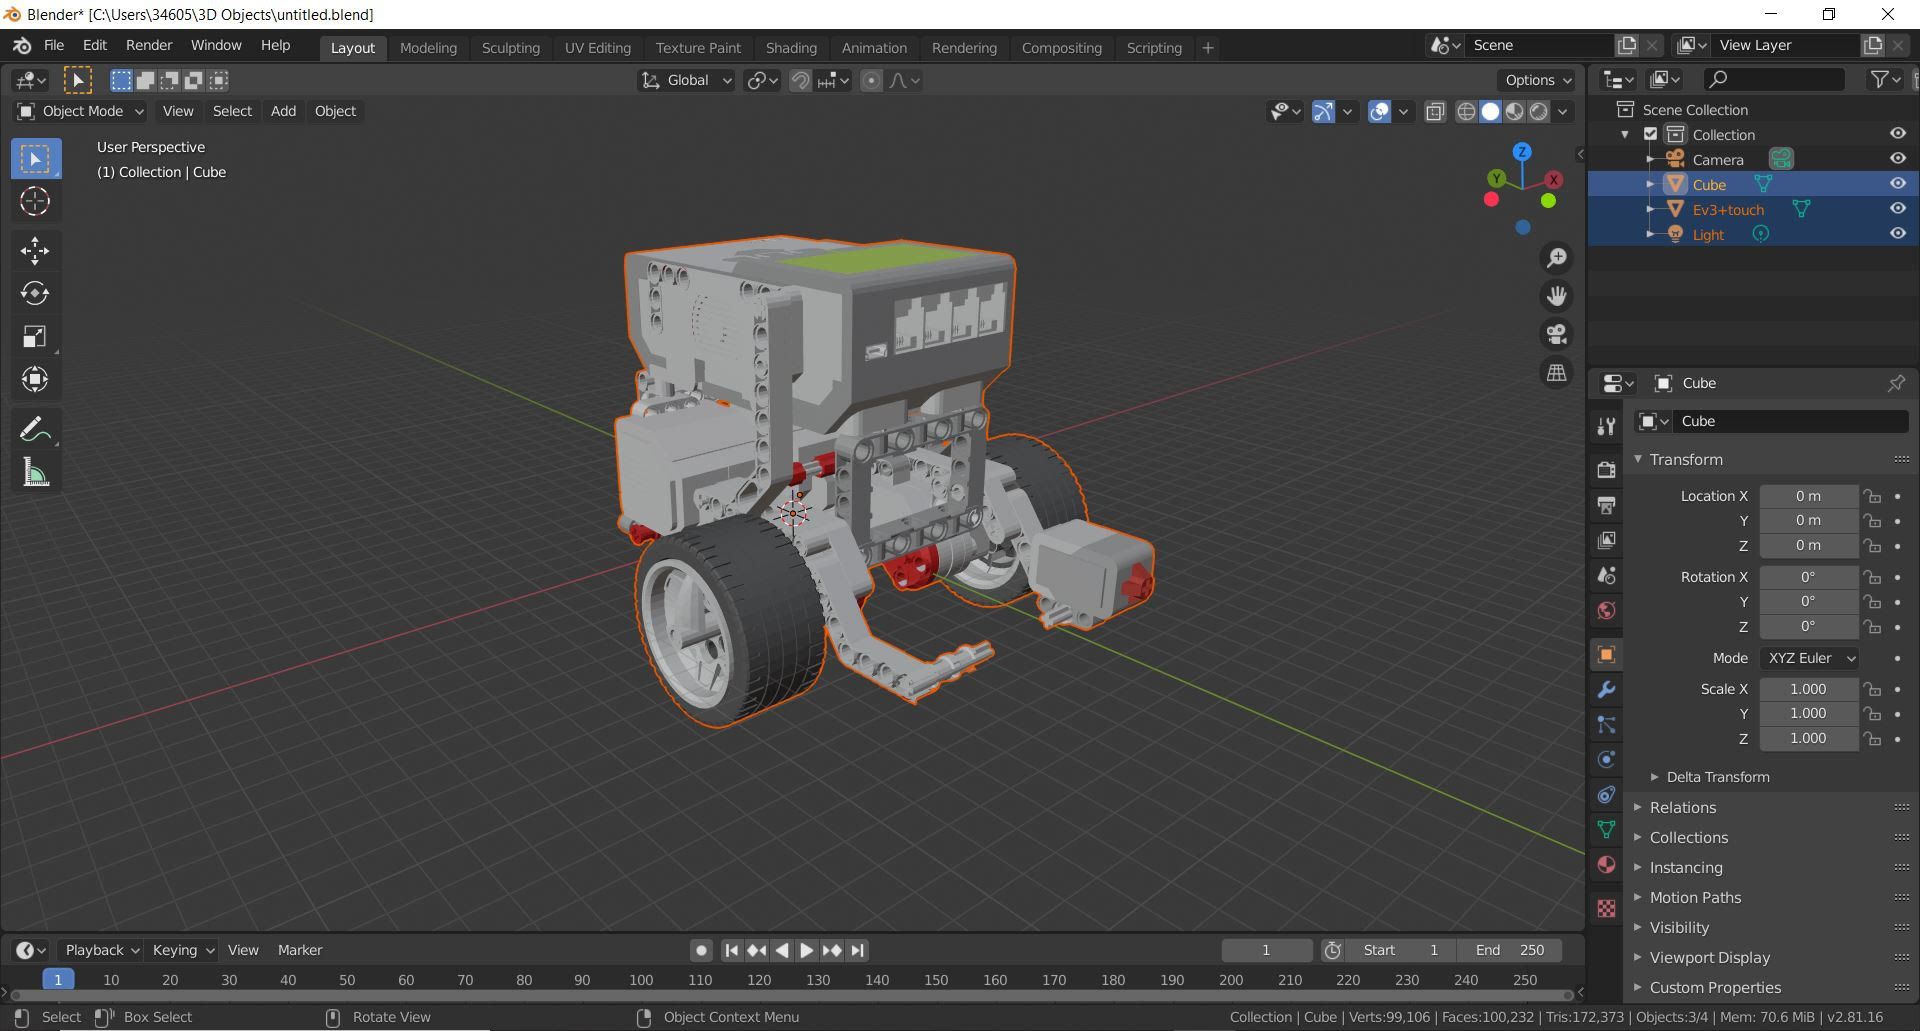
\includegraphics[width=0.7\textwidth]{img/blendertouch.jpg}
    \caption{Robot con sensor tactil} \label{fig:tactil}
\end{figure}
 \begin{figure}[H]
    \centering
    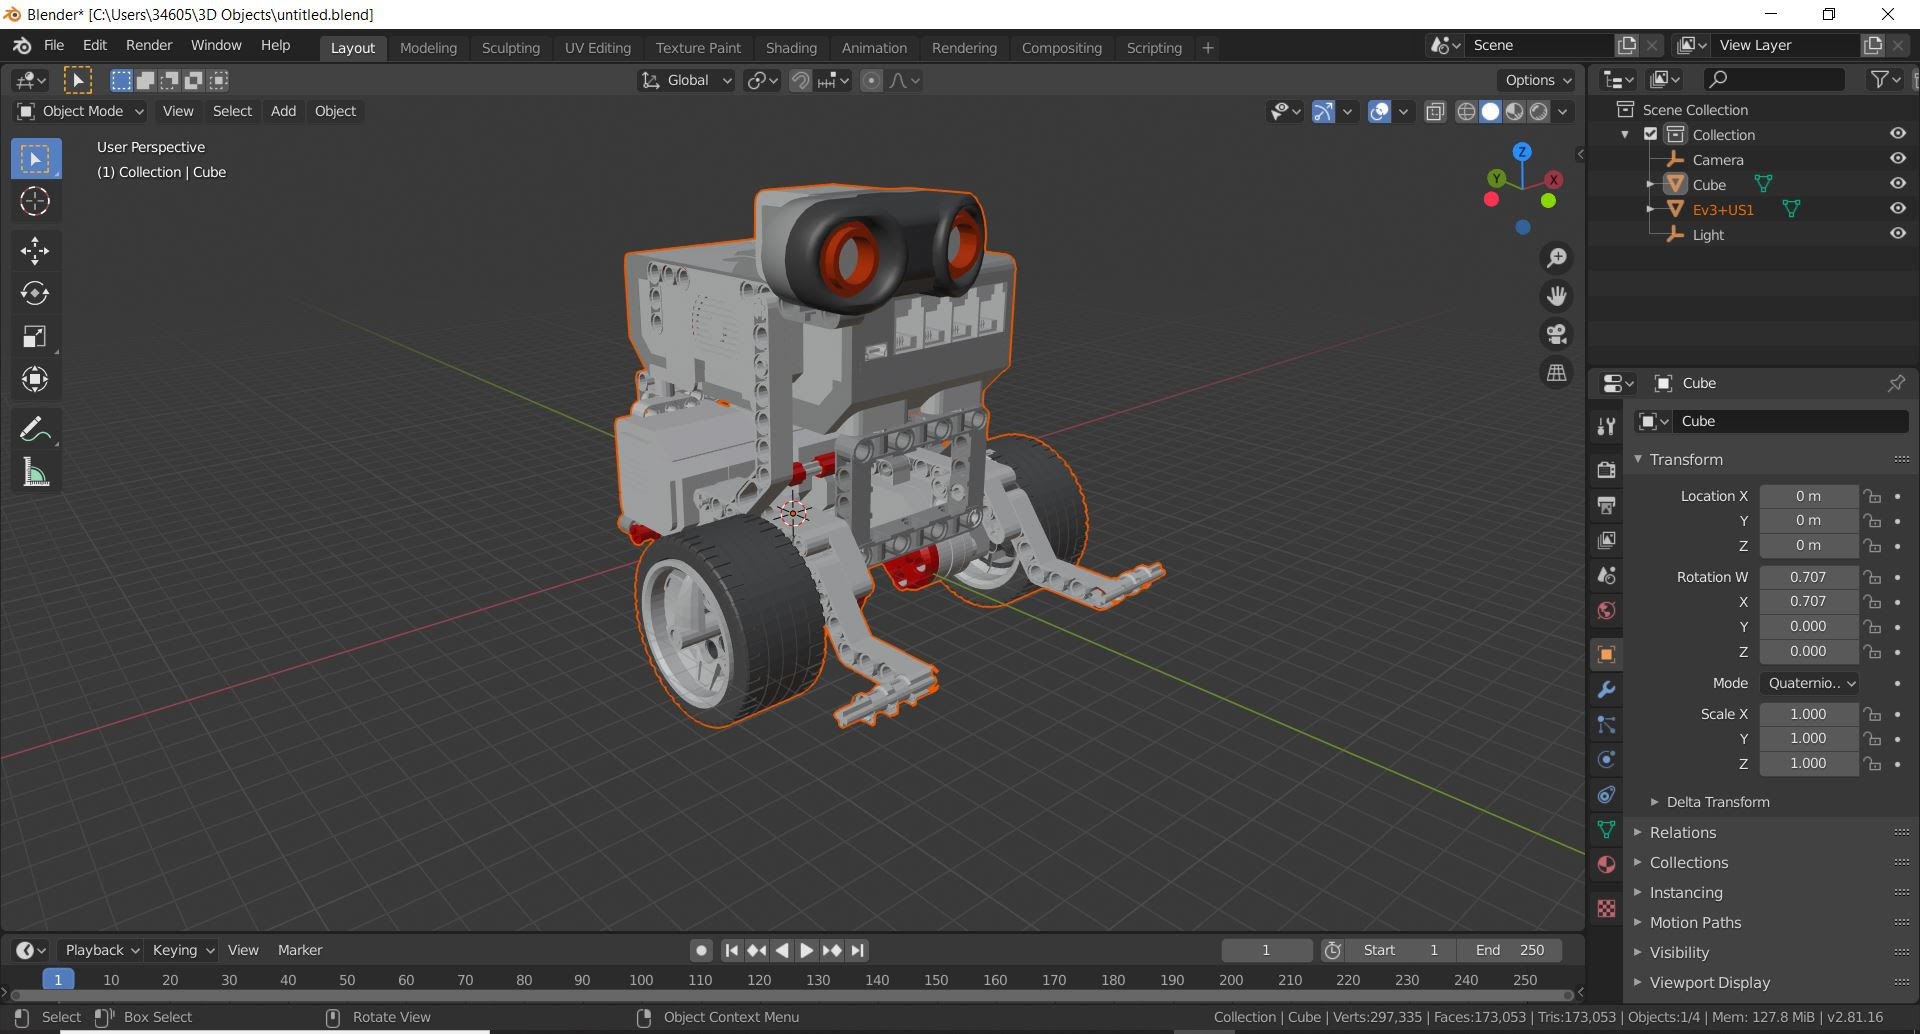
\includegraphics[width=0.7\textwidth]{img/blenderus.jpg}
    \caption{Robot con sensor de ultrasonidos} \label{fig:ultrasonidos}
\end{figure}


\section{Interfaz de programación de sensores y actuadores}
\sectionmark{Interfaz de programación}
\label{sec:interfazsimula}
\subsection{Soporte de actuadores}
Los motores son los actuadores del \textit{LEGO EV3}, son los que, a la orden del controlador, realizan el movimiento para completar su tarea asignada. En el kit de \textit{LEGO} vienen incluidos dos tipos de motores, motor grande y motor mediano.\newline
\begin{wrapfigure}{r}{0.3\linewidth}
    \centering
    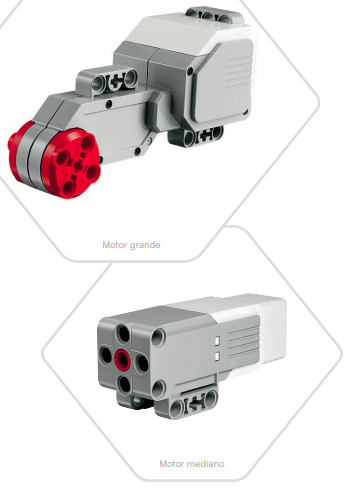
\includegraphics[width=0.6\linewidth]{img/motores.png}
    \caption{Motores}{{\footnotesize Actuadores que vienen incluidos}}
    \label{fig:color}
\end{wrapfigure}
 Los motores grandes, que son los que vamos a utilizar en el simulador, se suelen utilizar en pareja, para mover ambas ruedas del robot. A esto le llamamos \texttt{Tramo Diferencial} y se implementan las funciones pensando en este principio. Por ejemplo, si ejecutamos la función \textit{GirarDerecha()}, lo que va a ejecutar internamente es frenar el motor derecho, acelerar el motor izquierdo, y así hacer que el robot gire a la derecha. Este pensamiento nos ayuda a implementar el \textit{HAL API} de \textit{Kibotics} en este nuevo robot.  


\begin{table}[H]
  \begin{center}
    \caption{Métodos (HAL API) de los actuadores del robot.}
    \vspace{0.5cm}
    \label{tab:tablaMotores}
    \begin{tabular}{|c|c|} 
    \hline
      \textbf{Método} & \textbf{Descripción}\\
      \hline
.setV(integer) & \begin{tabular}[c]{@{}c@{}}Mueve hacia delante o atrás el robot.\\\end{tabular} \\ \hline
.setW(integer) & \begin{tabular}[c]{@{}c@{}}Hace girar al robot.\\\end{tabular} \\ \hline
.move(integer, integer) & \begin{tabular}[c]{@{}c@{}}Mueve el robot hacia delante/atrás y gira al mismo tiempo.\\ \end{tabular} \\ \hline
.getV() & \begin{tabular}[c]{@{}c@{}}Obtener la velocidad lineal configurada en el robot.\\ \end{tabular} \\ \hline
.getW() & \begin{tabular}[c]{@{}c@{}}Obtener la velocidad angular configurada en el robot.\\ \end{tabular} \\ \hline
    \end{tabular}
  \end{center}
\end{table}

Estas son las funciones que tiene el \textit{HAL API} y que ofrece el \textit{LEGO} simulado y que han sido programadas en \textit{JavaScript}.





\subsection{Soporte de sensores}
Se han analizado por separado los sensores para saber que funciones hay que añadir en los \textit{drivers}.
Estos \textit{drivers} están programados en \textit{JavaScript} permiten al usuario acceder a los sensores y obtener información del robot simulado.

\subsubsection{Sensor de color}
	 El Sensor de color es un sensor digital que puede detectar el color o la intensidad de la luz que ingresa por la pequeña ventana de la cara del sensor. Este sensor puede utilizarse en tres modos diferentes: Modo color, Modo intensidad de la luz reflejada y Modo intensidad de la luz ambiental.\newline
La tasa de muestreo del sensor de color es de 1 kHz.\newline
\begin{wrapfigure}{l}{0.3\linewidth}
    \centering
    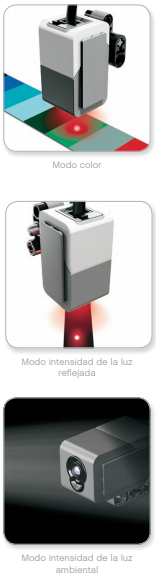
\includegraphics[width=0.6\linewidth]{img/color.png}
    \caption{Sensor color}{{\footnotesize Sensor de color en sus 3 usos}}
    \label{fig:color}
\end{wrapfigure}

\begin{itemize}
\item\textbf{En Modo color}, el Sensor de color reconoce siete colores: negro,
azul, verde, amarillo, rojo, blanco y marrón, además de Sin color. Esta capacidad de diferenciar los colores significa que su robot puede estar programado para clasificar pelotas o bloques de colores, y realizar acciones diferentes con cada color detectado.\newline
Este tipo de acciones, están ya contempladas en la funcionalidad del \textit{HAL API} de \textit{Kibotics}. Aunque en este caso utiliza una cámara simulada para comprobar qué color esta viendo.\newline
\textit{\textbf{getImage(cameraID)}}: Método que devuelve  \textit{robot}. 
    
    \begin{lstlisting}[language=javascript]
   function getImage(cameraID) {
    /**
     * Returns a screenshot from the robot camera
     */
    if (!cameraID || (this.camerasData.length === 1) || 
    (cameraID > this.camerasData.length - 1)) {
        return this.camerasData[0]['image'];
    } else {
        return this.camerasData[cameraID]['image'];
    }

}
    \end{lstlisting}
\end{itemize}

El \textit{LEGO EV3} no tiene una cámara instalada, pero para el robot simulado, es lo más sencillo de implementar, ya que puede analizar la imagen simulada y sacar el color RGB, para posteriormente dar nombre al color que ve.\newline
\textit{\textbf{getColorRGB()}}: Método que devuelve  \textit{RGB} en tres valores. 
    
    \begin{lstlisting}[language=javascript]
   function getObjectColorRGB(lowval, highval) {
    /**
     * This function filters an object in the scene with a given color, uses OpenCVjs to filter
     * by color and calculates the center of the object.
     *
     * Returns center: CenterX (cx), CenterY (cy) and the area of the object detected in the image.
     */

    if (lowval.length === 3) {
        lowval.push(0);
    }
    if (highval.length === 3) {
        highval.push(255);
    }
    var image = this.getImage();
    var binImg = new cv.Mat();
    var M = cv.Mat.ones(5, 5, cv.CV_8U);
    var anchor = new cv.Point(-1, -1);
    var lowThresh = new cv.Mat(image.rows, image.cols, image.type(), lowval);
    var highThresh = new cv.Mat(image.rows, image.cols, image.type(), highval);
    var contours = new cv.MatVector();
    var hierarchy = new cv.Mat();

    cv.morphologyEx(image, image, cv.MORPH_OPEN, M, anchor, 2,
        cv.BORDER_CONSTANT, cv.morphologyDefaultBorderValue()); // Erosion followed by dilation

    cv.inRange(image, lowThresh, highThresh, binImg);
    cv.findContours(binImg, contours, hierarchy, cv.RETR_CCOMP, cv.CHAIN_APPROX_SIMPLE);
    if (contours.size() > 0) {

        let stored = contours.get(0);
        var objArea = cv.contourArea(stored, false);

        let moments = cv.moments(stored, false);
        var cx = moments.m10 / moments.m00;
        var cy = moments.m01 / moments.m00;

    }
    return {center: [parseInt(cx), parseInt(cy)], area: parseInt(objArea)};
}
    \end{lstlisting}
    
Una vez realizado este paso podemos ponerle un nombre al color, como hace el \textit{LEGO EV3} real.

\begin{itemize}
\item\textbf{En Modo intensidad de la luz reflejada}, el Sensor de color mide la intensidad de la luz que se refleja desde una lámpara emisora de luz color rojo. El sensor utiliza una escala de 0 (muy oscuro) a 100 (muy luminoso). Esto significa que su robot puede estar programado para moverse sobre una superficie blanca hasta detectar una línea negra o para interpretar una tarjeta de identificación con código de color.
Esto en el robot simulado, es diferente, ya que no podemos ver como una magnitud física como es la luz se refleja un objeto, pero este efecto depende del color que se esté viendo en la imagen, la luminosidad del color se puede calcular con esta función:

\textit{\textbf{getLightness(valuemin, valuemax)}}: Método que devuelve  \textit{Luminosidad}. 
    
    \begin{lstlisting}[language=javascript]
   function getLightness(valuemin, valuemax) {
    
    let image = this.getObjectColorRGB(valuemin, valuemax);
    let L = ((image.center[0]- image.center[1])/2)*100/255;
    
    /**
     * Returns lightness with a percent
     */
    
    return L.

}
\end{lstlisting}

Esta funcion puede resultar util, para, por ejemplo, poder seguir una linea, cuando haya colores muy similares, o cuando se esté utilizando el robot en una mesa o superficie alta, detectar antes, donde está el borde.

\item\textbf{En Modo intensidad de la luz ambiental}, el Sensor de color mide la intensidad de la luz que ingresa en la ventana desde su entorno, como la luz del sol o el haz de una linterna. El sensor utiliza una escala de 0 (muy oscuro) a 100 (muy luminoso). Esta funcionalidad, no puede ser implementada en la plataforma, ya que no tenemos un foco de luz que se puede analizar, ni tampoco una magnitud dentro del entorno que represente la luz.

\end{itemize}

\subsubsection{Sensor de ultrasonido}

El Sensor ultrasónico es un sensor digital que puede medir la distancia a un objeto que se encuentra frente a él. Para hacerlo, envía ondas de sonido de alta frecuencia y mide cuánto tarda el sonido en reflejarse de vuelta al sensor. La frecuencia de sonido es demasiado alta para el oído humano.
La distancia a un objeto puede medirse en pulgadas o centímetros.\newline
\begin{wrapfigure}{r}{0.5\linewidth}
    \centering
    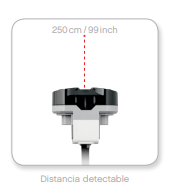
\includegraphics[width=0.5\linewidth]{img/ultrasonidos.png}
    \caption{Sensor de ultrasonidos}
    \label{fig:ultrasonido}
\end{wrapfigure}
Esto le permite programar su robot para que se detenga a una distancia determinada de una pared. Al utilizar unidades en centímetros, la distancia detectable es entre 3 y 250 centímetros (con una exactitud de +/- 1 centímetro). Un valor de 255 centímetros significa que el sensor no puede
detectar ningún objeto frente a él.\newline
En \textit{WebSim} la implementación que hay para las distancias es  usar un \textit{RayCaster}. Que es equivalente a poner láseres apuntando hacia todas direcciones por delante del robot de esta forma:

\begin{figure}[H]
    \centering
    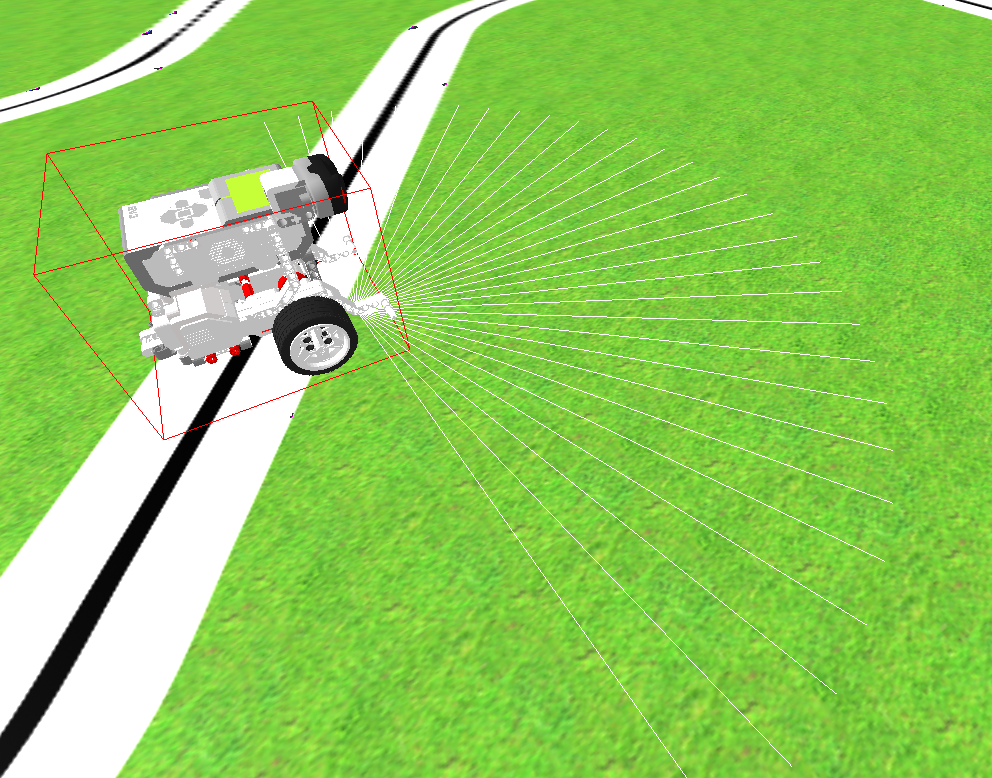
\includegraphics[width=0.7\textwidth]{img/pruebaUS.png}
    \caption{Raycaster} \label{fig:raycaster}
\end{figure}

Lo cual devuelve un \textit{array} de valores con las distancias a las que "rebota" cada láser. Esto tratándose de un sensor ultrasonidos que solo devuelve un único valor con el obstáculo más cercano, es un poco irreal. Por lo que creare la función \textit{getDistance} que devuelve el valor más cercano de todos los que hay en el \textit{array} de \textit{RayCaster} 

\textit{\textbf{Funciones que calculan la distancia}}: Método que devuelve  un único valor con la distancia más corta. 

 \begin{lstlisting}[language=javascript]
function getDistance() {
    /**
     * This function returns the distance for the raycaster in the center of the arc of rays.
     */
    var distances = this.getDistances();

    if (distances[13] !== 10 || distances[14] !== 10 || distances[15] !== 10 || distances[16] !== 10 || distances[17] !== 10) {
        let distance0 = 100;
        let distance1 = 100;
        let distance2 = 100;
        let distance3 = 100;
        let distance4 = 100;
        if (distances[13] !== 10) {
            distance0 = distances[13];
        }
        if (distances[14] !== 10) {
            distance1 = distances[14];
        }
        if (distances[15] !== 10) {
            distance2 = distances[15];
        }
        if (distances[16] !== 10) {
            distance3 = distances[16];
        }
        if (distances[17] !== 10) {
            distance4 = distances[17];
        }
        let min_distances = [distance0, distance1, distance2, distance3, distance4];
        Array.min = function (array) {
            return Math.min.apply(Math, array);
        };
        return Array.min(min_distances);
    } else {
        return 10;
    }
}

function getDistances() {
    /**
     * This function returns an array with all the distances detected by the rays.
     */
    var distances = [];
    for (var i = 0; i <= 31; i++) {
        distances.push(10);
    }
    var groups = ["center", "right", "left"];
    for (i = 0; i < groups.length; i++) {
        this.distanceArray[groups[i]].forEach((obj) => {
            if (typeof obj.d != "undefined") {
                distances[obj.id] = obj.d;
            }
        });
    }
    return distances;
}
\end{lstlisting}

\subsubsection{Sensor de contacto}

El Sensor táctil es un sensor analógico que puede detectar el momento en el que se presiona y se lanza el botón rojo del sensor. Esto significa que el Sensor táctil puede programarse para actuar según tres condiciones: presionado, lanzado o en contacto (tanto presionado como lanzado). Con la información del Sensor táctil se puede programar un robot para ver el mundo como lo haría una persona no vidente, es decir, extendiendo un brazo y respondiendo cuando toca algo (presionado).
\begin{wrapfigure}{r}{0.5\linewidth}
    \centering
    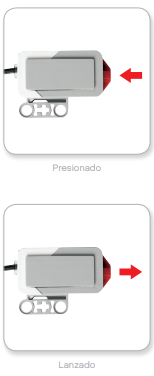
\includegraphics[width=0.5\linewidth]{img/tactil.png}
    \caption{Sensor tactil}
    \label{fig:tactil}
\end{wrapfigure}
Se puede construir un robot con un Sensor táctil presionado contra la superficie. Luego, puede programar el robot para que responda (se detenga) cuando esté a punto de pasar el borde de la mesa (cuando el sensor se lanza). Un robot de pelea puede programarse para continuar empujando hacia adelante en dirección a su oponente hasta que este se retire. Ese par de acciones, presionado y lanzado, constituyen el estado En contacto.

En la plataforma no había ninguna función similar que implementara un sensor de contacto. Así que, se han creado un par de funciones, que aprovechándose del \textit{array} de distancias, cogerán la distancia central y cuando sea mínima, darán por hecho que el robot está tocando la superficie

   \begin{lstlisting}[language=javascript]
     getCenterDistance(){
      
      if (this.distanceArray["center"][0] != null) {
          return this.distanceArray["center"][0].d;
      } else {
          return 10;
      }
    }
    isTouching() {
        return (this.getCenterDistance()<3);
    }
\end{lstlisting}

Esta función al ser totalmente nueva, habrá que añadirla en el \textit{HAL API} , el cual esta programado en \textit{JavaScript} y tendrá que tener su equivalente en \textit{Python} y en \textit{Blockly}, esto significa que hay que traducirla en diferentes idiomas y añadirla a la lista de bloques que son visibles en el editor visual. Esta implementación la mostrare en la siguiente parte con la prueba de este sensor en un ejercicio.

\subsubsection{Girosensor}
El Girosensor es un sensor digital que detecta el movimiento de rotación en un eje simple. Si rota el Girosensor en la dirección que indican las flechas que se encuentran en la caja del sensor, este puede detectar la razón de rotación en grados por segundo. (El sensor puede medir una razón de giro máxima de 440 grados por segundo.) Entonces, puede utilizar la razón de rotación para detectar, por ejemplo, si gira una parte del robot o si el robot se cae.

\begin{wrapfigure}{l}{0.5\linewidth}
    \centering
    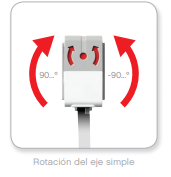
\includegraphics[width=0.5\linewidth]{img/gyrosensor.png}
    \caption{girosensor}
    \label{fig:girosensor}
\end{wrapfigure}

Además, el Girosensor registra el ángulo de rotación total en grados. Puede utilizar este ángulo de rotación para detectar, por ejemplo,cuánto ha girado su robot. Esta función le permite programar giros (sobre el eje que está midiendo el Girosensor) con una exactitud de +/- 3 grados en un giro de 90 grados.

Este sensor no requiere una implementación dentro de la plataforma ya que el único uso que puede darse dentro de la plataforma, es medir un giro de unos grados que pasas como argumentos. Y eso ya está implementado en el \textit{HAL API}. El otro uso real que se le puede dar a este sensor es para que un robot mantenga el equilibrio dinámico, mientras se mueve. Pero los tres montajes elegidos de \textit{LEGO Ev3} para implementar en \textit{Kibotics} no tienen un centro de gravedad en el mantenerse.

  
\section{Validación experimental con ejercicios}
\sectionmark{Validación experimental}
\label{sec:ejercicios}

Se han añadido ejercicios para comprobar la funcionalidad de cada uno de los sensores anteriormente explicados 

\subsection{Sigue-líneas}
    Este ejercicio consiste en seguir una línea negra en el suelo sobre fondo blanco haciendo uso de la cámara del \textit{robot}, que recoge las imágenes y las filtra para poder seguirla.
    
    
    \begin{figure}[H]
    \centering
    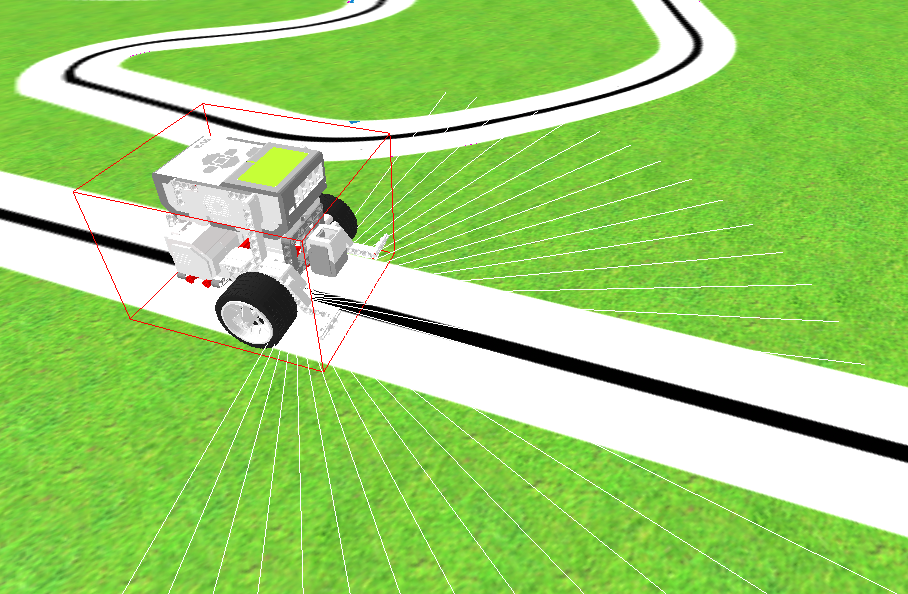
\includegraphics[scale=0.4]{img/siguelineas.png}
    \caption{Escenario para el ejercicio \textit{LEGO EV3} sigue-líneas} \label{fig:siguelinea}
    \end{figure}
    
        \begin{figure}[H]
    \centering
    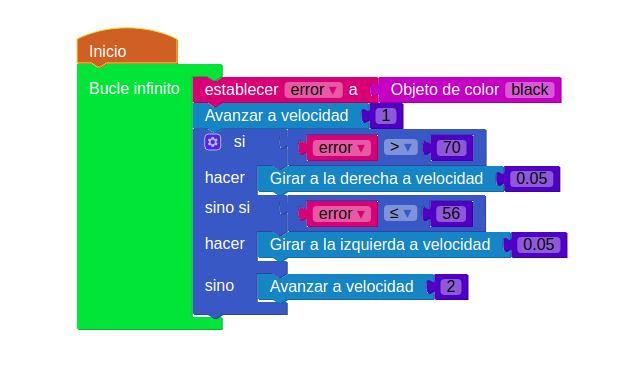
\includegraphics[scale=0.5]{img/solucion.png}
    \caption{Solución en \textit{Scratch} para el ejercicio sigue-líneas} 
    \label{fig:solucion}
    \end{figure}
    
En la solución se establece un error con el color negro, de modo que dependiendo del lado por el que me pase, corrijo girando hacia al lado contrario. En este ejemplo utilizo una actualización de funciones que ya existían, por lo que puedo programarlas en \textit{Blockly}, habiendo hecho solo cambios en el \textit{HAL API} que está programado en \textit{JavaScript} para el robot \textit{LEGO Ev3}.
    
    
\subsection{Choca-gira}
\label{subsec:chocagira}
En este ejercicio hay programar al \textit{robot} para que avance recto mientras no haya obstáculos haciendo uso del sensor de ultra-sonidos. Si encuentra un obstáculo tiene que detenerse, retroceder un poco, girar a la derecha y seguir adelante.


    \begin{figure}[H]
    \centering
    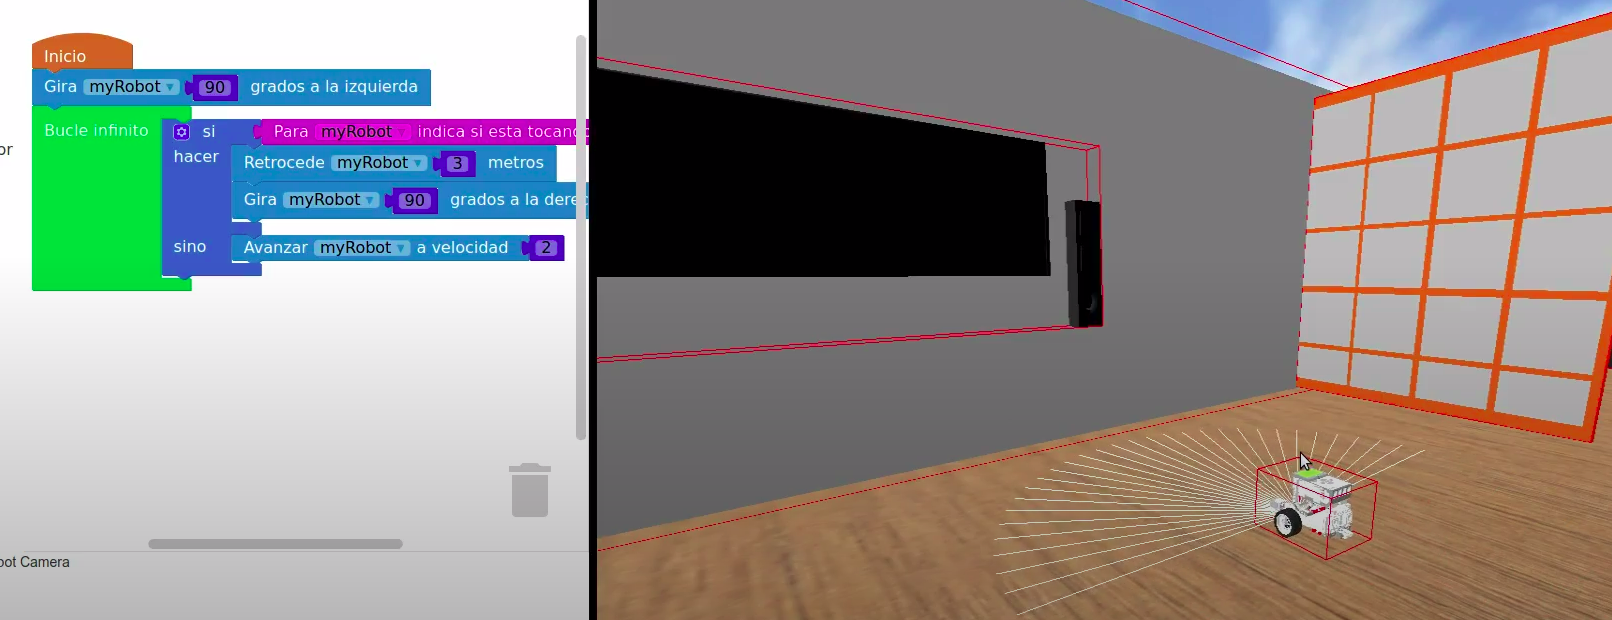
\includegraphics[scale=0.25]{img/chocagira.png}
    \caption{Solución en \textit{Scratch} para el ejercicio choca-gira} 
    \label{fig:chocagira}
    \end{figure}
    
    En esta solución\footnote{\url{https://youtu.be/figTbXKEXD4}} se prueba el bloque anteriormente mencionada que equivale a la funcion \textit{IsTouching} en el lenguaje \textit{Scratch}. Cabe destacar que aquí estamos  utilizando la nueva función que se ha creado para este sensor. En este caso, estamos utilizando el bloque "Para \textbf{myRobot} indica si está tocando" que es el bloque de \textit{Blockly} equivalente a la función \textit{IsTouching} en \textbf{JavaScript} del \textit{HAL API}
    
\subsection{Atraviesa-bosque}
\label{subsec:atraviesabosque}
Ejercicio basado en atravesar un pasillo con diversos objetos que hay que esquivar. El sensor necesario es el ultrasonidos para detectar en qué posición se encuentra el siguiente obstáculo. Este ejercicio solo se puede hacer simuladamente, ya que el \textit{LEGO EV3} con el sensor ultrasonido no puede saber en qué posición se encuentra el obstáculo, solo la distancia. Aún así, este ejercicio tiene un gran interés educativo, por lo que he decidido añadirlo, y ademas crear una nueva función para que sea más sencillo e intuitivo de completar para el estudiante.

\textit{\textbf{GetMinorDistance}}: Método que devuelve en que dirección se encuentra el obstáculo más cercano. 

 \begin{lstlisting}[language=javascript]
 getMinorDistance() {
      /*
        This function returns the minor distance of an array with all distances
      */

      var distances = []
      let ray = 32;
      let distance=5;
      for (var i = 0; i <= 31; i++) {
          distances.push(10);
      }
      var groups = ["center", "right", "left"];
      for (var i = 0; i < groups.length; i++) {
          this.distanceArray[groups[i]].forEach((obj) => {
              if (typeof obj.d != "undefined") {
                  distances[obj.id] = obj.d;
              }
          });
      }
      for (var i=0; i<distances.length; i++){
        if (distances[i]<distance){
          distance=distance[i]
          ray=i;
        }
      }
      if (ray > 15 && ray < 32) {
          return groups[1];

      }else if(ray == 15){
          return groups[0];

      } else if (ray < 15) {
          return groups[2];

      }else {
          return "unhindered";
      }
    }
 
 
 \end{lstlisting}

Con esta función se puede resolver el ejercicio con un simple bucle que distingue entre las tres opciones que devuelve.

    \begin{figure}[H]
    \centering
    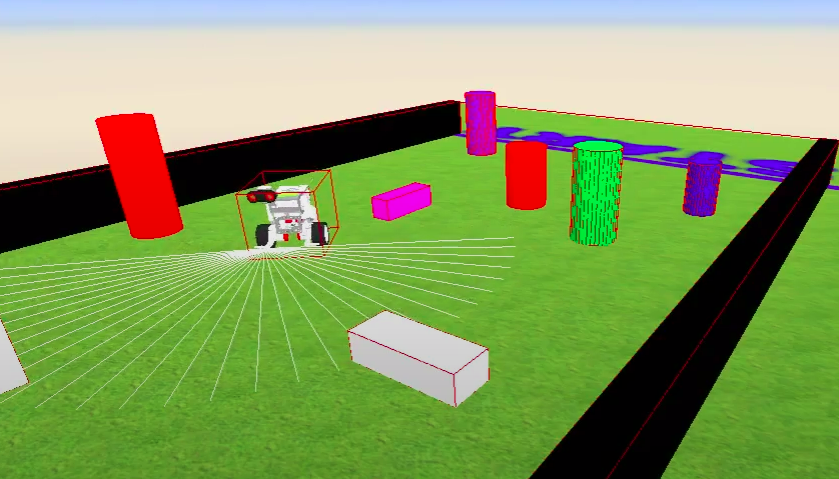
\includegraphics[scale=0.45]{img/forest.png}
    \caption{Escenario para el ejercicio atraviesa bosque} 
    \label{fig:atraviesaBosque}
    \end{figure}

    \begin{figure}[H]
    \centering
    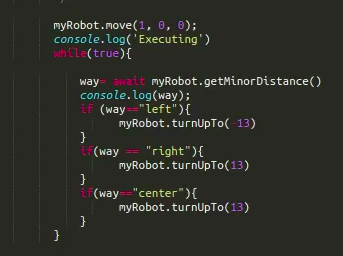
\includegraphics[scale=0.6]{img/solucionforest.png}
    \caption{Solución en \textit{JavaScript} para el ejercicio atraviesa bosque} 
    \label{fig:solucionforest}
    \end{figure}
    
    En esta solución\footnote{\url{https://youtu.be/ZSYWMSSRkS8}} se obtienen todos los valores que devuelve el sensor de ultra-sonidos y, según donde detecte el obstáculo, gira en un sentido u otro. Este último ejemplo está programado en \textit{JavaScript} ya que está función no esta implementada en el \textit{HAL API} y no tiene equivalentes en \textit{Blockly} ni \textit{Python}


